\section{Marco Teorico}

\begin{frame}{Inteligencia Artificial y ML}
  \begin{itemize}
    \item Busqueda de \textbf{agentes} capaces de tomar la decision correcta en funcion de la información disponible.
  \end{itemize}

  \begin{block}{Aprendizaje automático (\textbf{Machine Learning})}
    Un programa de computadora aprende de la experiencia E con repecto a alguna clase de tareas T y una medida de desempeño P, si su desempeño en tareas de T, medidio por P, mejora con la experiencia E.
  \end{block}
  Segun el tipo de experiencia y medida de desempeño, se divide en:
  
    \begin{itemize}
      \item Aprendizaje supervisado
      \item Aprendizaje no supervisado
      \item \textbf{Aprendizaje por refuerzo}
    \end{itemize}
\end{frame}

\begin{frame}{Aprendizaje por Refuerzo (RL)}
  \begin{columns}[T,onlytextwidth]

    % ---- Columna izquierda: texto ----
    \column{0.50\textwidth}
    Un agente interactúa con un entorno dinámico donde:
    \begin{itemize}
        \item Observa estados $s_t$
        \item Ejecuta acciones $a_t$
        \item Recibe recompensas $r_{t+1}$
    \end{itemize}

    \vspace{0.2cm}
    Con el objetivo de maximizar la recompensa final acumulada:
    \[
    \max_\pi \ \mathbb{E}[R]
    \]

    Principales desafíos:
    \begin{itemize}
        \item Problema de asignación de crédito
        \item Exploración vs explotación
        \item Retroalimentación escasa y diferida
    \end{itemize}

    % ---- Columna derecha: imagen ----
    \column{0.50\textwidth}
    \begin{center}
      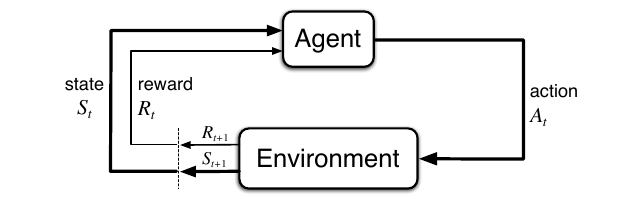
\includegraphics[
        width=\linewidth,
        height=0.75\textheight,
        keepaspectratio
      ]{./attatchments/interaccion_rl.png}
    \end{center}
  \end{columns}
\end{frame}

\begin{frame}{Procesos de Decisión de Markov (MDP)}
    La interaccion \textbf{Agente-Entorno} se formaliza mediante un MDP.
    \begin{block}{Proceso de Decision de Markov}
        Se define como una tupla $...$, donde:
        \begin{itemize}
            \item S
            \item A
            \item P
            \item R
            \item \gamma
        \end{itemize}
    \end{block}

    \begin{block}{Propiedad de Markov}
        El estado actual $s_t$ contiene la informacion necesaria para estimar la posible evolucion del entorno.
    \end{block}
\end{frame}

\begin{frame}{Componentes del Aprendizaje por Refuerzo}
    El Agente toma acciones siguiendo una \textbf{Política}: mapeo de estados y observaciones del entorno a una accion que debera tomar el agente.
    
    \textbf{Objetivo del agente}: encontrar la politica que maximice el retorno final.

    \begin{block}{Retorno y Politica Optima}
        Dado una secuencia de recompensas $r_{t+1},r_{t+2}\cdots$, se define el retorno como:
        $$
        G_t = \sum_{k=0}^{T-t-1} {\gamma^k r_{t+k+1}}
        $$

        La politica optima sera $\pi^\ast = \arg\max_{\pi} J(\pi)$ donde
        $J(\pi) = \mathbb{E}[G_0]$
    \end{block}
\end{frame}

\begin{frame}{Componentes del Aprendizaje por Refuerzo}
    \begin{block}{Ecuaciones de Bellman}
        Ecuaciones recursivas que nos permiten estimar la recompensa esperada segun la situacion actual del Agente en el entorno.
        
        \begin{itemize}
            \item \textbf{Función de valor de estado}: estima la recompensa acumulada esperada al partir del estado $s$ y seguir la política $\pi$.
                \begin{itemize}
                    \item $V^\pi(s) = \mathbb{E}_\pi \left[ r_{t+1} + \gamma V^\pi(S_{t+1}) \mid S_t = s \right]$
                \end{itemize}
            \item \textbf{Función de valor de acción} estima la recompensa acumulada esperada tras ejecutar la acción $a$ en el estado $s$ y continuar siguiendo $\pi$.
                \begin{itemize}
                    \item $Q^\pi(s,a) = \mathbb{E}_\pi \left[ r_{t+1} + \gamma Q^\pi(S_{t+1}, A_{t+1}) \mid S_t = s, A_t = a \right]$.
                \end{itemize} 
        \end{itemize}
    \end{block}

    En espacios de accion continuos:
    \begin{itemize}
        \item Computar $\arg\max_a Q(s,a)$ no es factible
        \item Se aproximan dichas funciones mediante redes neuronales
    \end{itemize}
\end{frame}
 

%Como en la slide anterioor ya deje la idea de que dichas ecuaciones no son posibles de caluclar en espacios continuos, ahora quiero primero dar una idea de la taxonomia y familias de algoritmos de Deep Rl, oralmente explicando que todos consisten de utilizar Redes neuronales como aproximadores de la funcion objetivo. En algunos sera la funcion Q, en otros la politica y para el caso actor critico ambos.

%Luego una diapositiva introduciendo el concepto de los metodos Actor critico, y como se aproximan las funciones con redes: 
%Q ≈ Q(s,a;θ)
%π ≈ π(s;θ)

%Y luego continuaremos con Redes recurrentes, dependencia temporal, BPTT y de ahi se desprende la idea de utilizar TD3 + BPTT. Finalmente se dara la inspiracion biologica, el TWC y el desafio tecnico. Pero por el momento estas diapositivas no las armemos.

\begin{frame}{Algoritmos de RL}
  \centering
    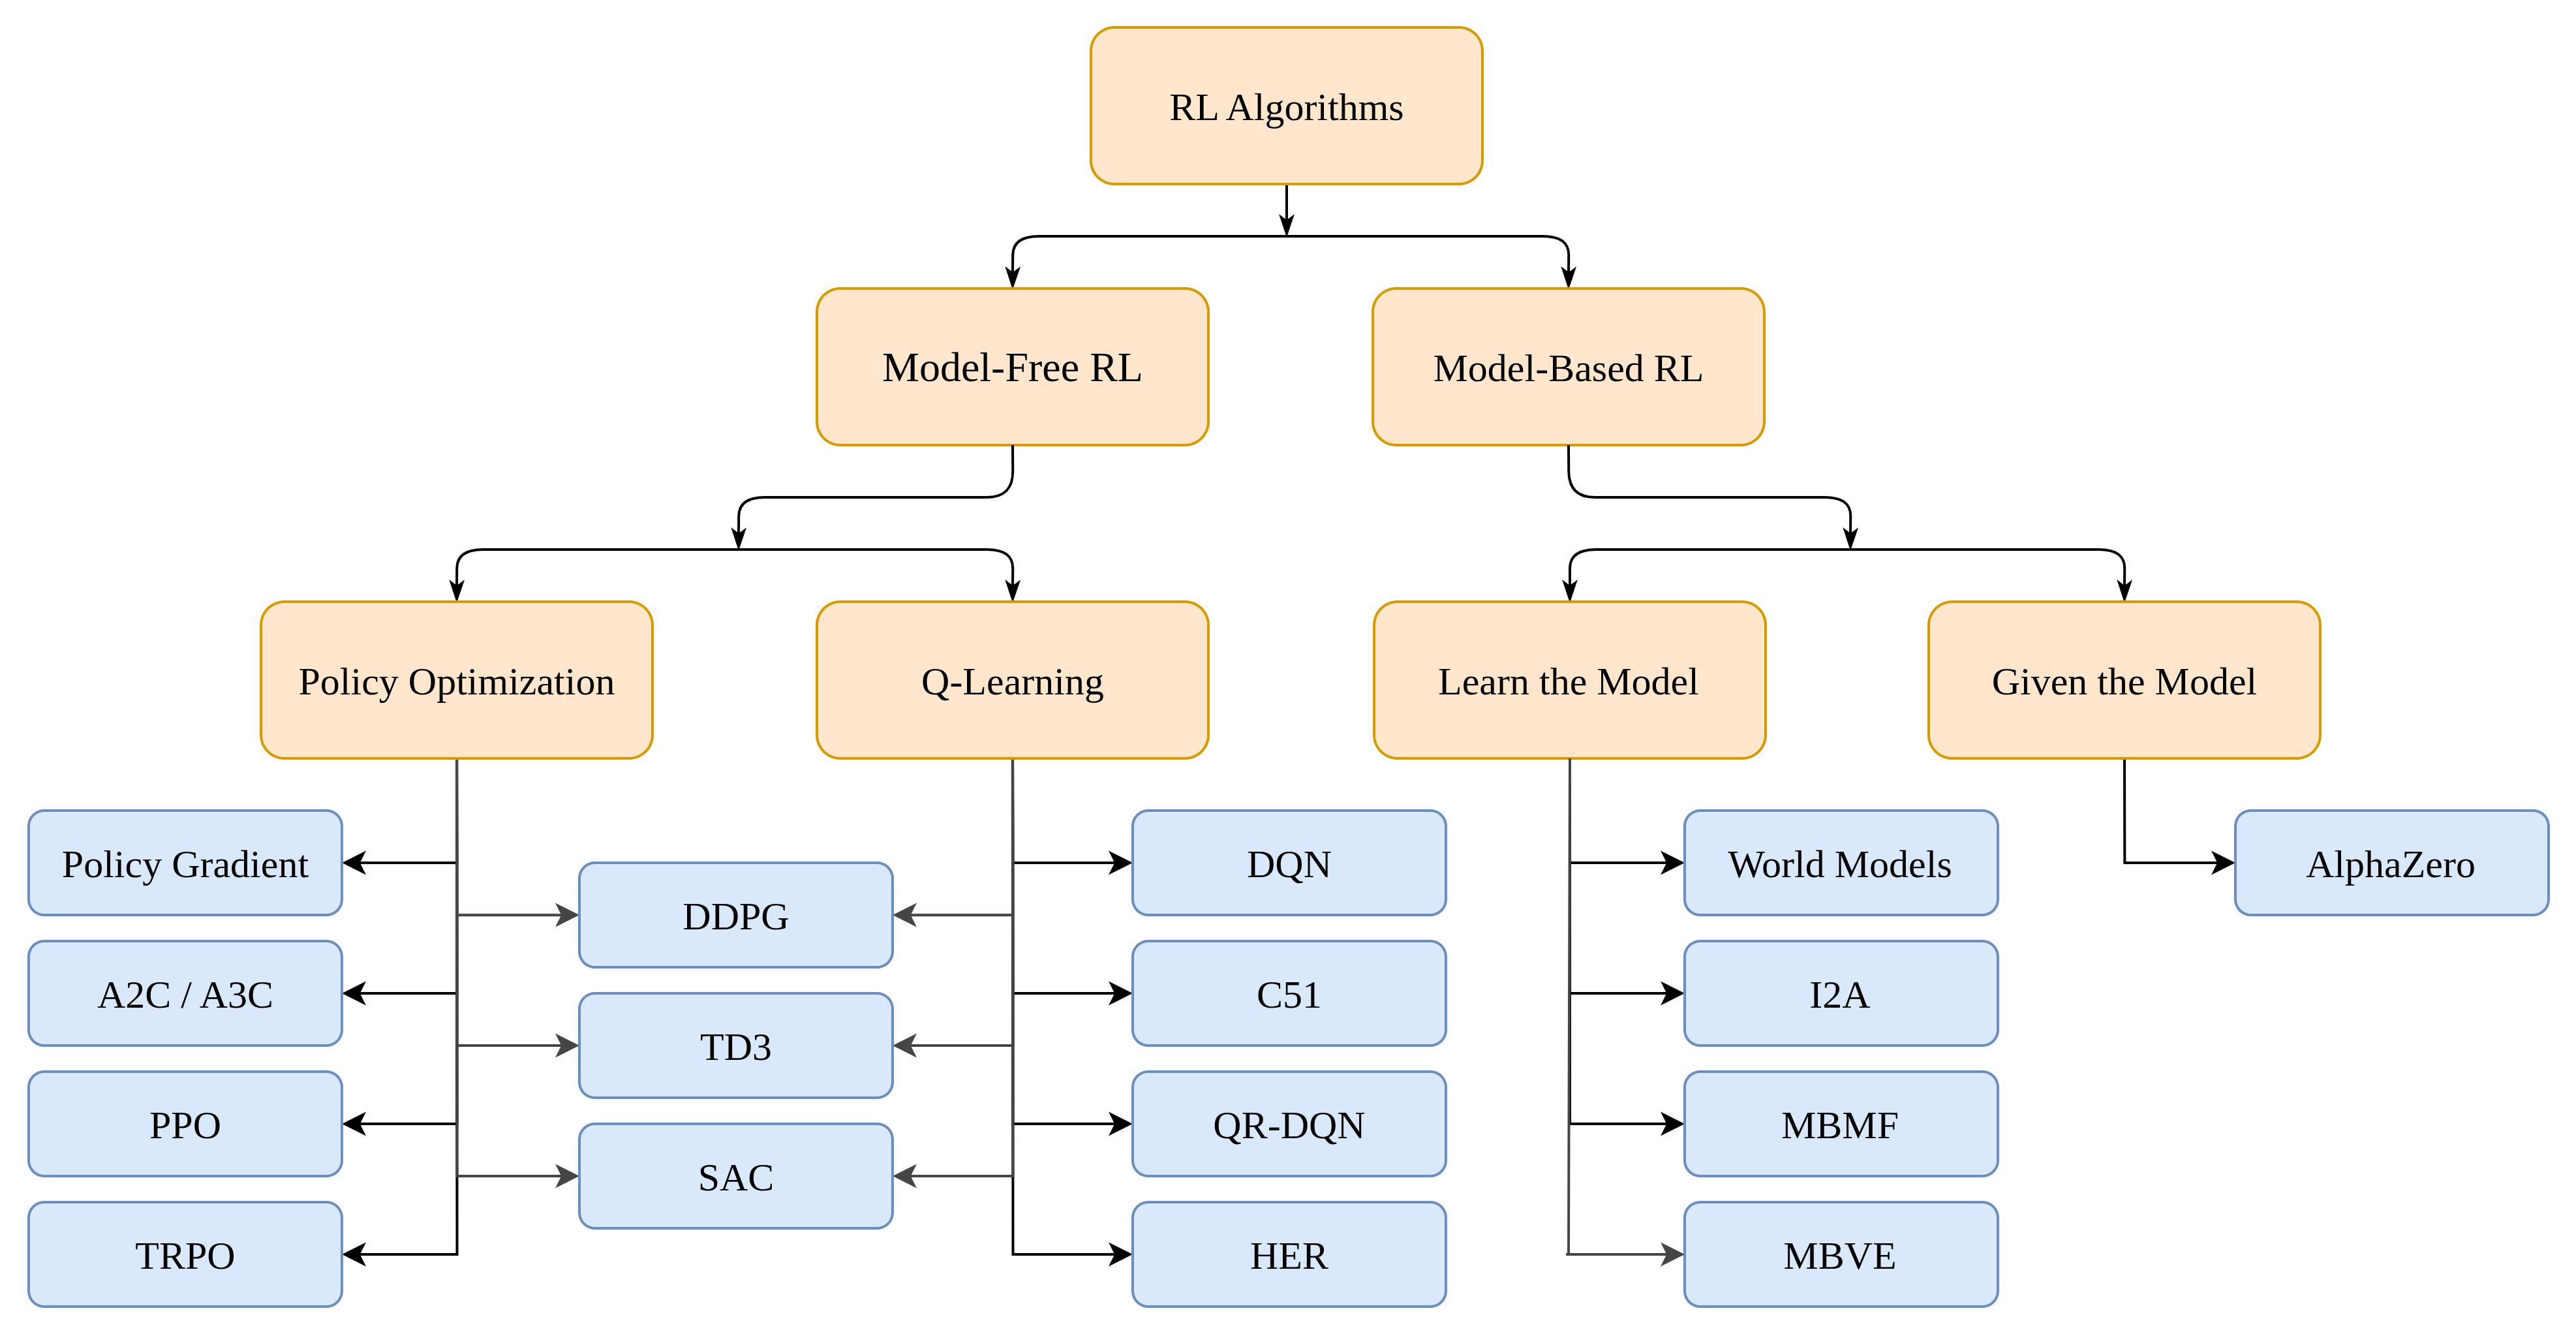
\includegraphics[
      width=\linewidth,
      height=0.85\textheight,
      keepaspectratio
    ]{./attatchments/rl_algorithms.png}
\end{frame}

\begin{frame}{Redes Neuronales}
  \begin{columns}[T,onlytextwidth]

    % ---- Columna izquierda: texto ----
    \column{0.40\textwidth}
      \begin{itemize}
        \item Comunmente utilizadas como aproximadores de funciones universales.
        \item Se entrenan mediante metodos basados en el \textbf{descenso por el gradiente}. 
      \end{itemize}
      \vspace{0.4cm}
      \[
        \theta \leftarrow \theta - \alpha \nabla_\theta L(\theta)
      \]

    % ---- Columna derecha: imagen ----
    \column{0.60\textwidth}
      \begin{center}
        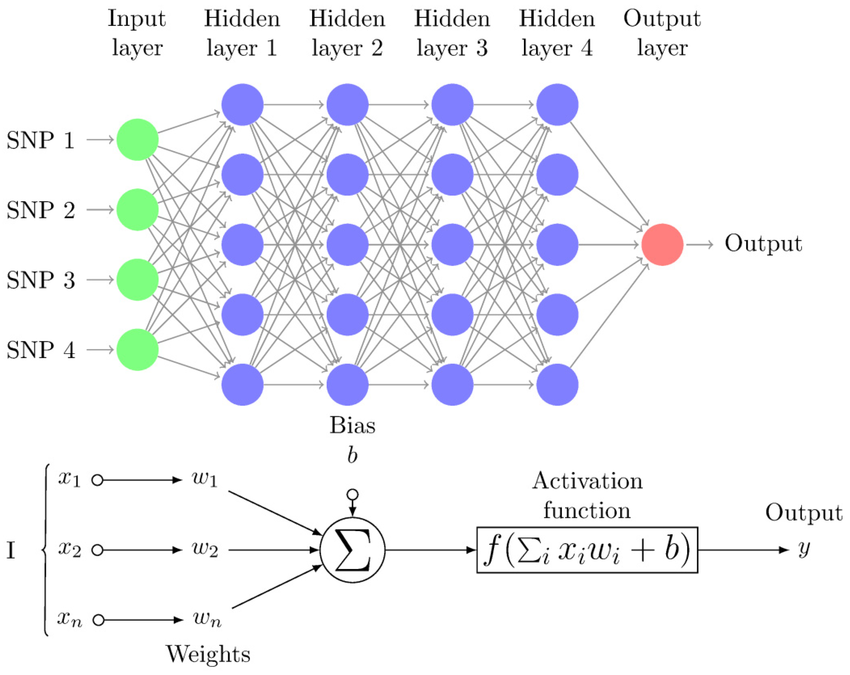
\includegraphics[
          width=\linewidth,
          height=0.75\textheight,
          keepaspectratio
        ]{./attatchments/mlp.png}
      \end{center}
  \end{columns}
\end{frame}


\begin{frame}{Dinamica Neuronal FIU}
  \begin{columns}[T,onlytextwidth]
    \column{0.50\textwidth}

    % Compactar SOLO las ecuaciones (no toda la slide)
    {\small
    \setlength{\abovedisplayskip}{2pt}
    \setlength{\belowdisplayskip}{2pt}
    \setlength{\jot}{2pt}

    \begin{equation*}
      \begin{aligned}
        S_n &= E_n + \sum_{j=1}^{m} I_{in}^{j}
      \end{aligned}
    \end{equation*}

    \begin{equation*}
      O_n =
      \begin{cases}
        S_n - T_n, & \text{si } S_n > T_n \\
        0,         & \text{en otro caso}
      \end{cases}
    \end{equation*}

    \begin{equation*}
      E_n =
      \begin{cases}
        S_n - T_n, & \text{si } S_n > T_n \\
        E_n - d_n, & \text{si } S_n \le T_n \ \land\  S_n = E_n \\
        S_n,       & \text{en otro caso}
      \end{cases}
    \end{equation*}

    \begin{equation*}
      I_{in}^{j} =
      \begin{cases}
        \ \omega_j O_j, & \text{gap junc. y } O_j \ge E_n \\
        -\omega_j O_j,  & \text{gap junc. y } O_j < E_n \\
        \ \omega_j O_j, & \text{exc. química} \\
        -\omega_j O_j,  & \text{inh. química}
      \end{cases}
    \end{equation*}
    } % end \small

    \column{0.50\textwidth}
    TODO: Ilustracion de una neurona o como fue implementada (placeholder)
  \end{columns}
\end{frame}

\begin{frame}{La arquitectura TWC}
  \centering
    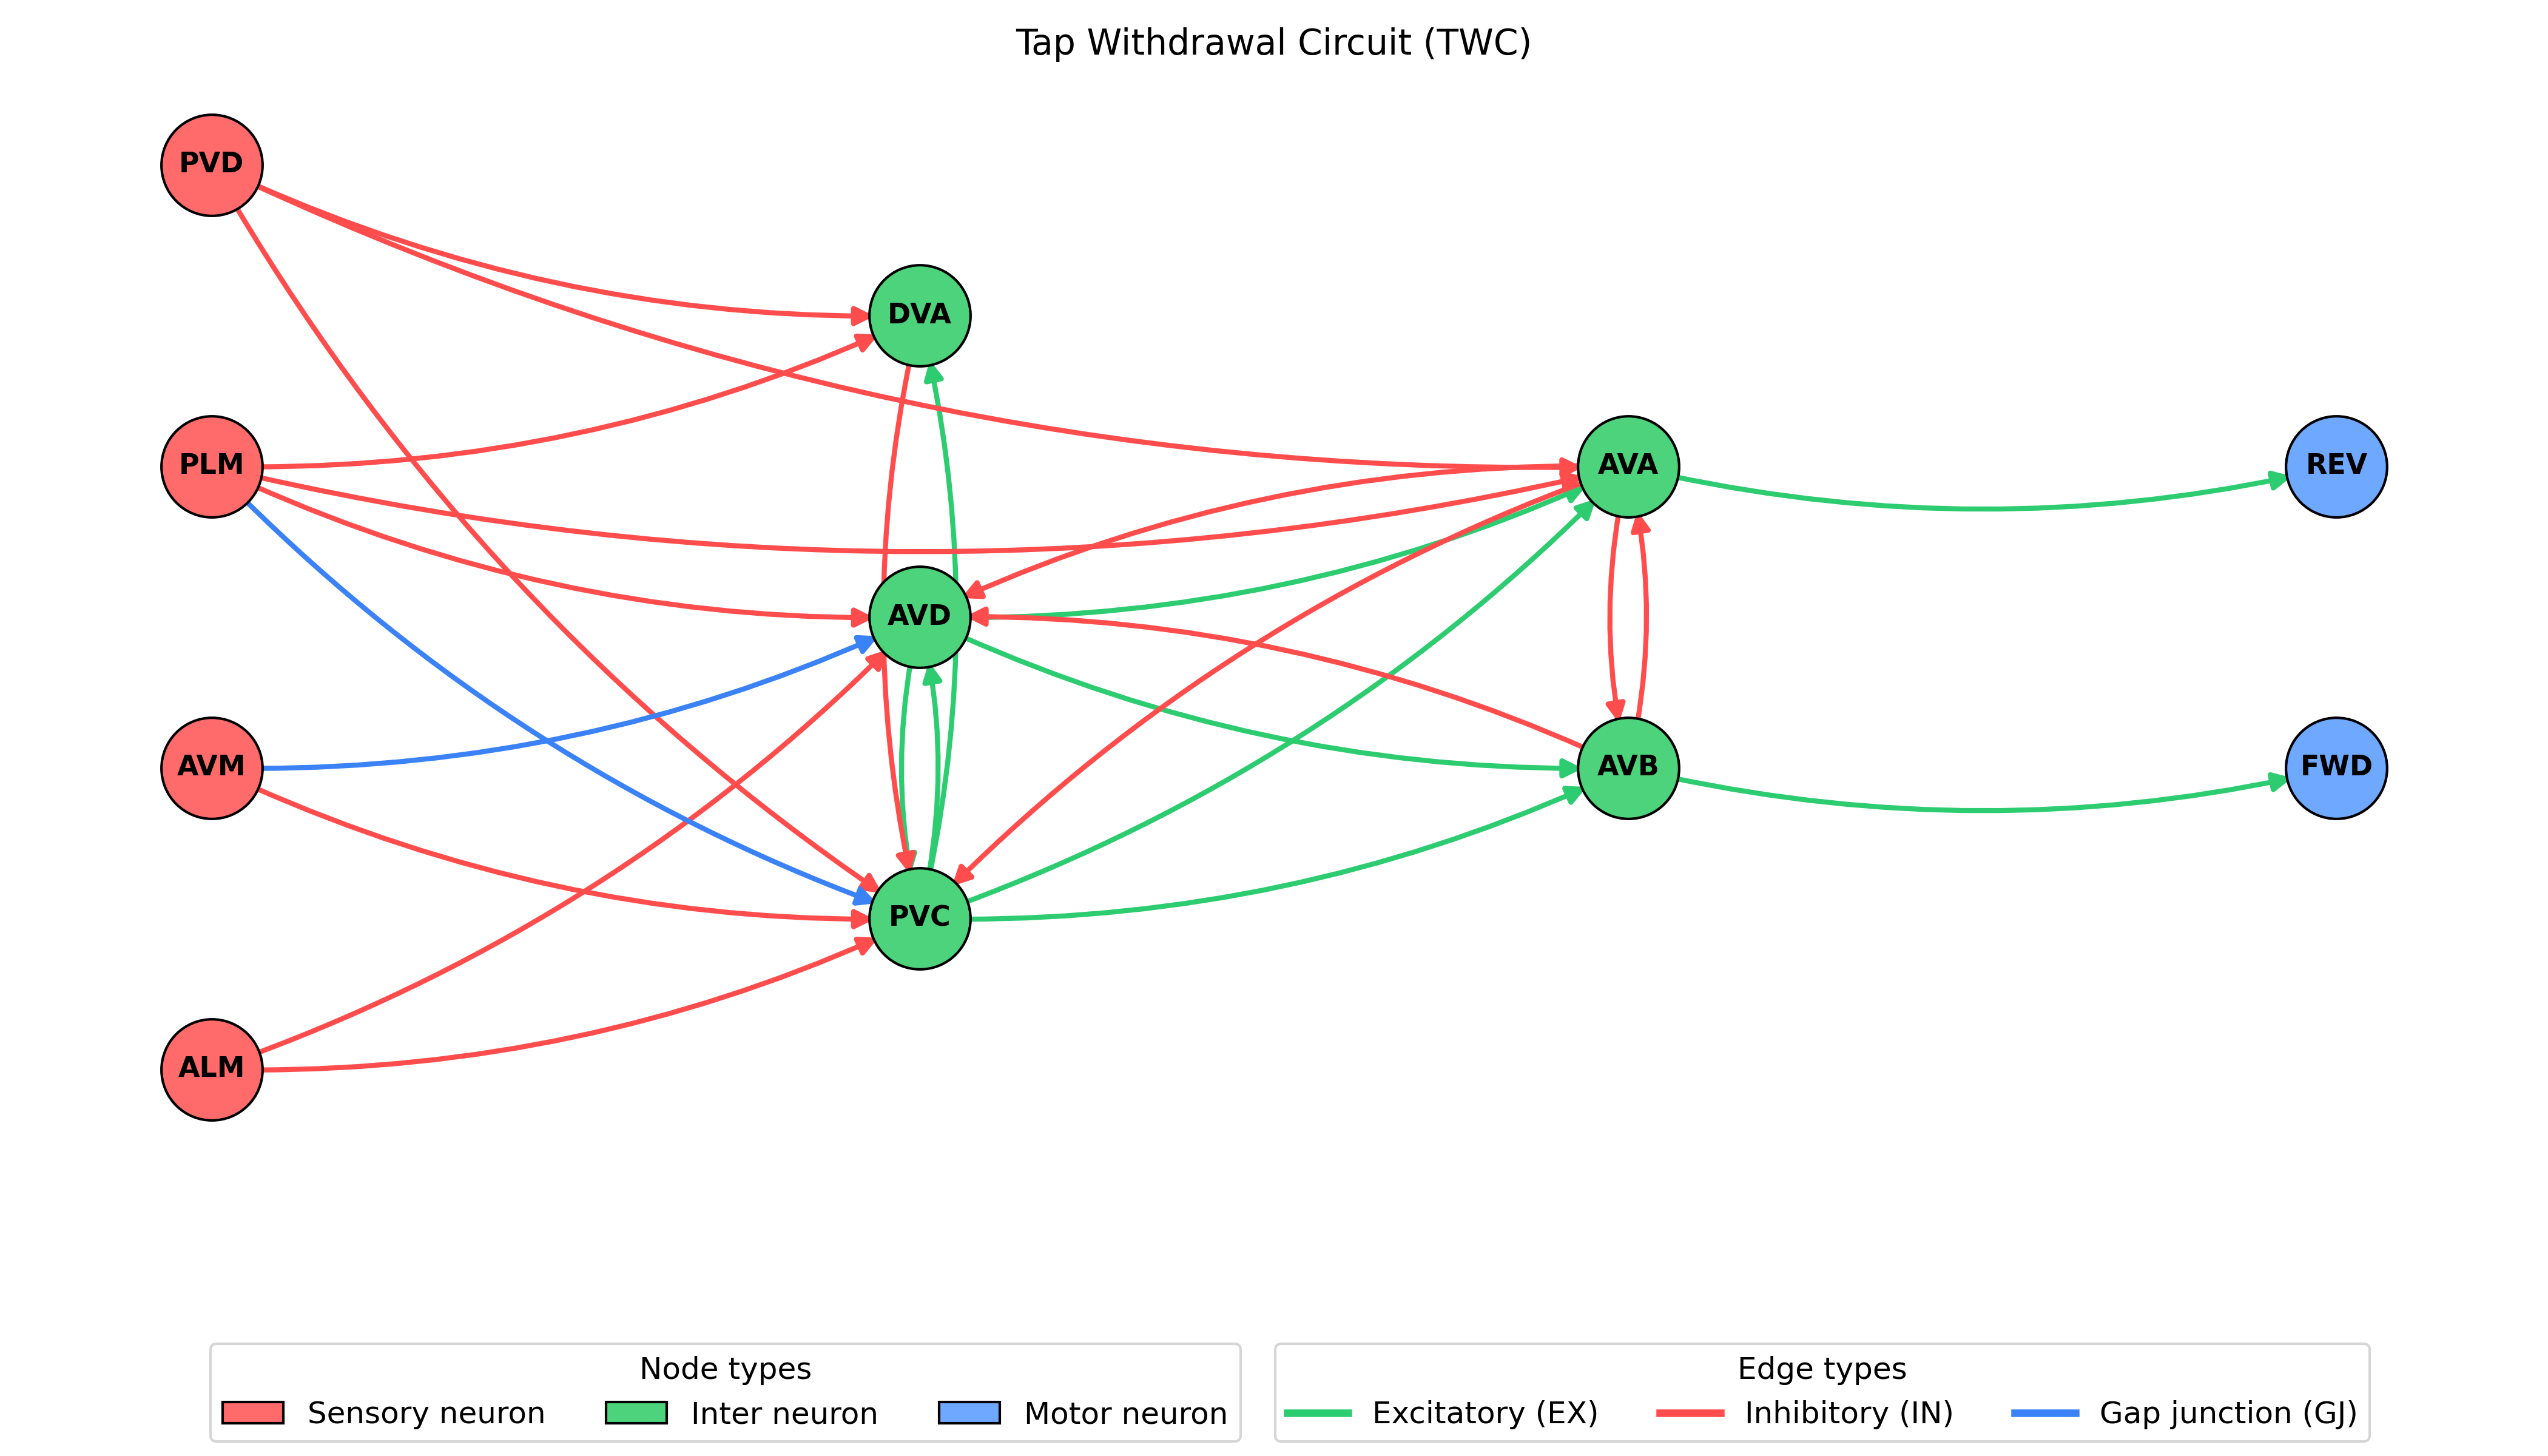
\includegraphics[
      width=\linewidth,
      height=0.82\textheight,
      keepaspectratio
    ]{./attatchments/twc.png}
\end{frame}
